%% Supplement to nhess_manuscript.tex (uploaded as a separate PDF to NHESS).
%% Copernicus publishes supplements as supplied, so this file uses the standard article class.
%% References to the main text (equations) are hard-coded.

\documentclass[11pt,a4paper]{article}

\usepackage[T1]{fontenc}
\usepackage{times}
\usepackage[margin=2.5cm]{geometry}
\usepackage{amsmath}
\usepackage{graphicx}
\usepackage{booktabs}
\usepackage[authoryear,round]{natbib}
\usepackage[hidelinks]{hyperref}

\renewcommand{\thefigure}{S\arabic{figure}}
\renewcommand{\thetable}{S\arabic{table}}

\title{Supplement of\\[0.5em]
\textbf{Multi-hazard scenario ensembles for estimating earthquake risk}}
\author{Alexandre Dunant, Tom R. Robinson, Alexander L. Densmore, Sweata Sijapati, Nick J. Rosser,\\
Mark Kincey, Katie J. Oven, Stine Heiselberg, and Ragindra Man Rajbhandari}
\date{\textit{Correspondence to:} Alexandre Dunant (alexandre.dunant@eurac.edu)}

\begin{document}

\maketitle

\noindent This Supplement contains Figs.~S1--S5 and Tables~S1--S2, which are referred to in the main text.

\clearpage

\begin{figure}[p]
\centering
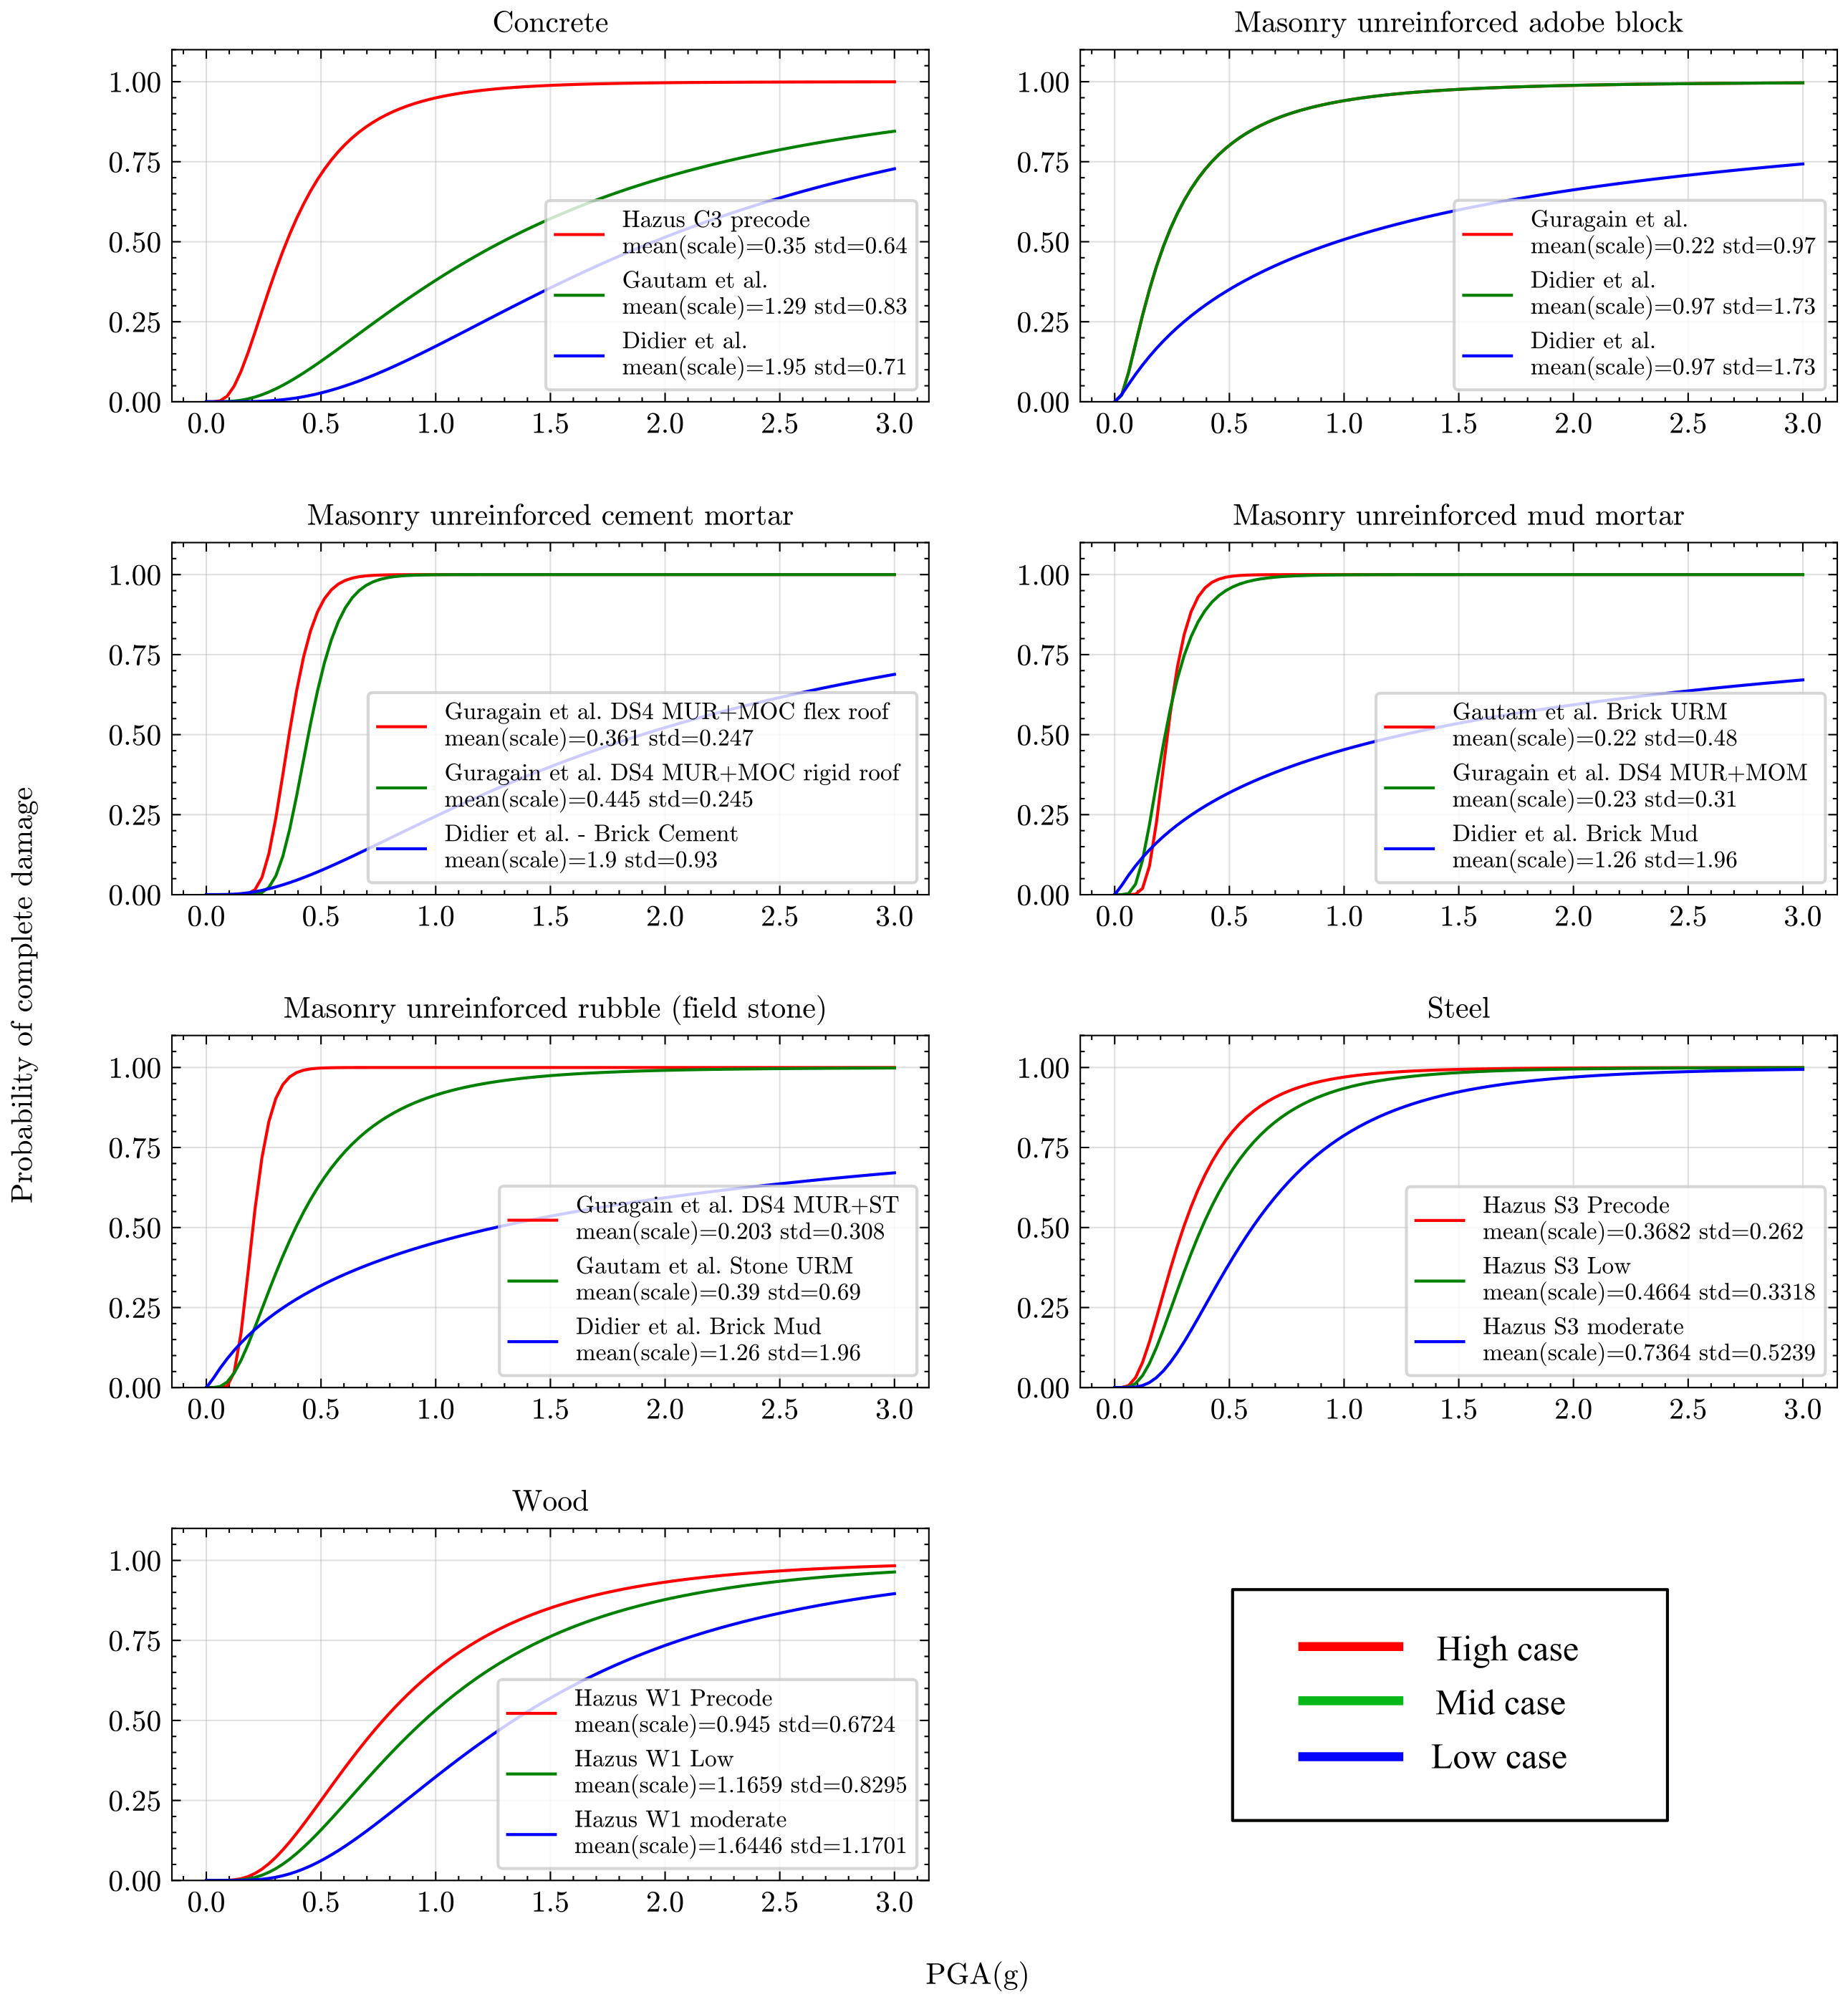
\includegraphics[width=\textwidth]{figures/figS1.png}
\caption{Fragility functions used in the hypergraph network modelling, modified from \citet{Dunant2025}. Each panel shows the functions for a different building type in the METEOR dataset (\url{https://maps.meteor-project.org/map/building-exposure-map-of-nepal}), relating peak ground acceleration (PGA, in g) to the probability of a complete damage state. Note that each fragility function is defined by two parameters: a scale parameter that sets the PGA value for 50\,\% probability of complete damage, and a standard deviation (std) that defines the spread of the curve. Parameter values and sources for the fragility curves are included in the plots \citep{FEMA2020Hazus, Didier2017, Gautam2018, Guragain2021}. For the experiments shown here, we adopt the mid case for each building type; see \citet{Dunant2025} for discussion.}
\label{fig:S1}
\end{figure}

\begin{figure}[p]
\centering
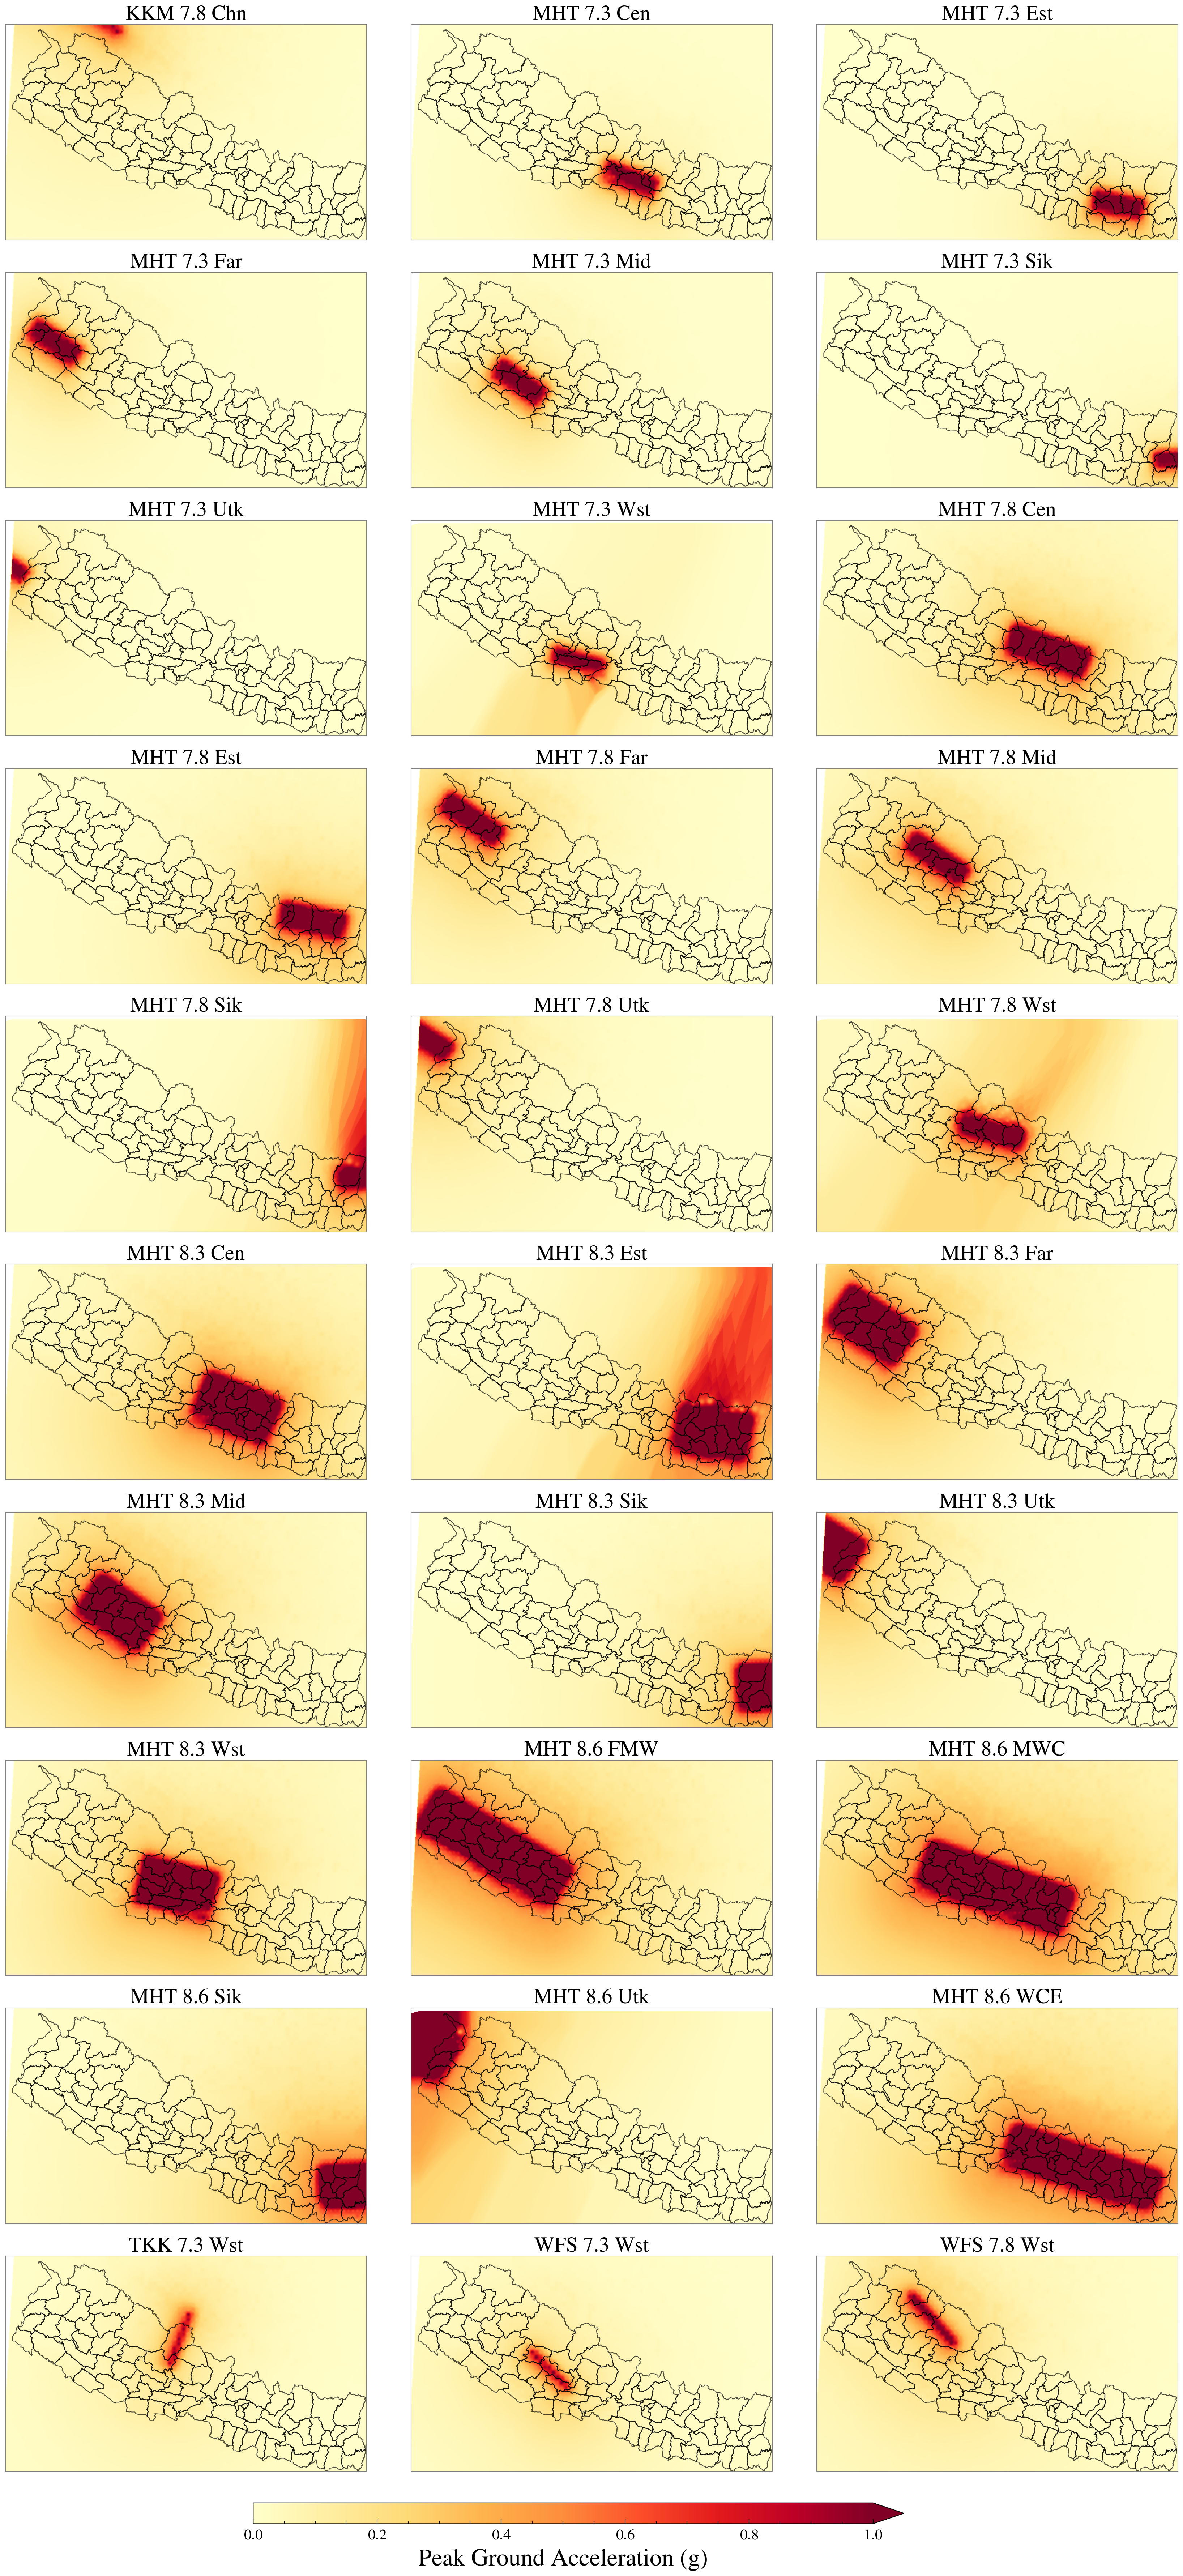
\includegraphics[width=\textwidth,height=0.82\textheight,keepaspectratio]{figures/figS2.png}
\caption{Maps of peak ground acceleration (PGA, in g) for each of the 30 scenario earthquakes in the ensemble. Earthquake name codes match those defined by \citet{Robinson2018}.}
\label{fig:S2}
\end{figure}

\begin{figure}[p]
\centering
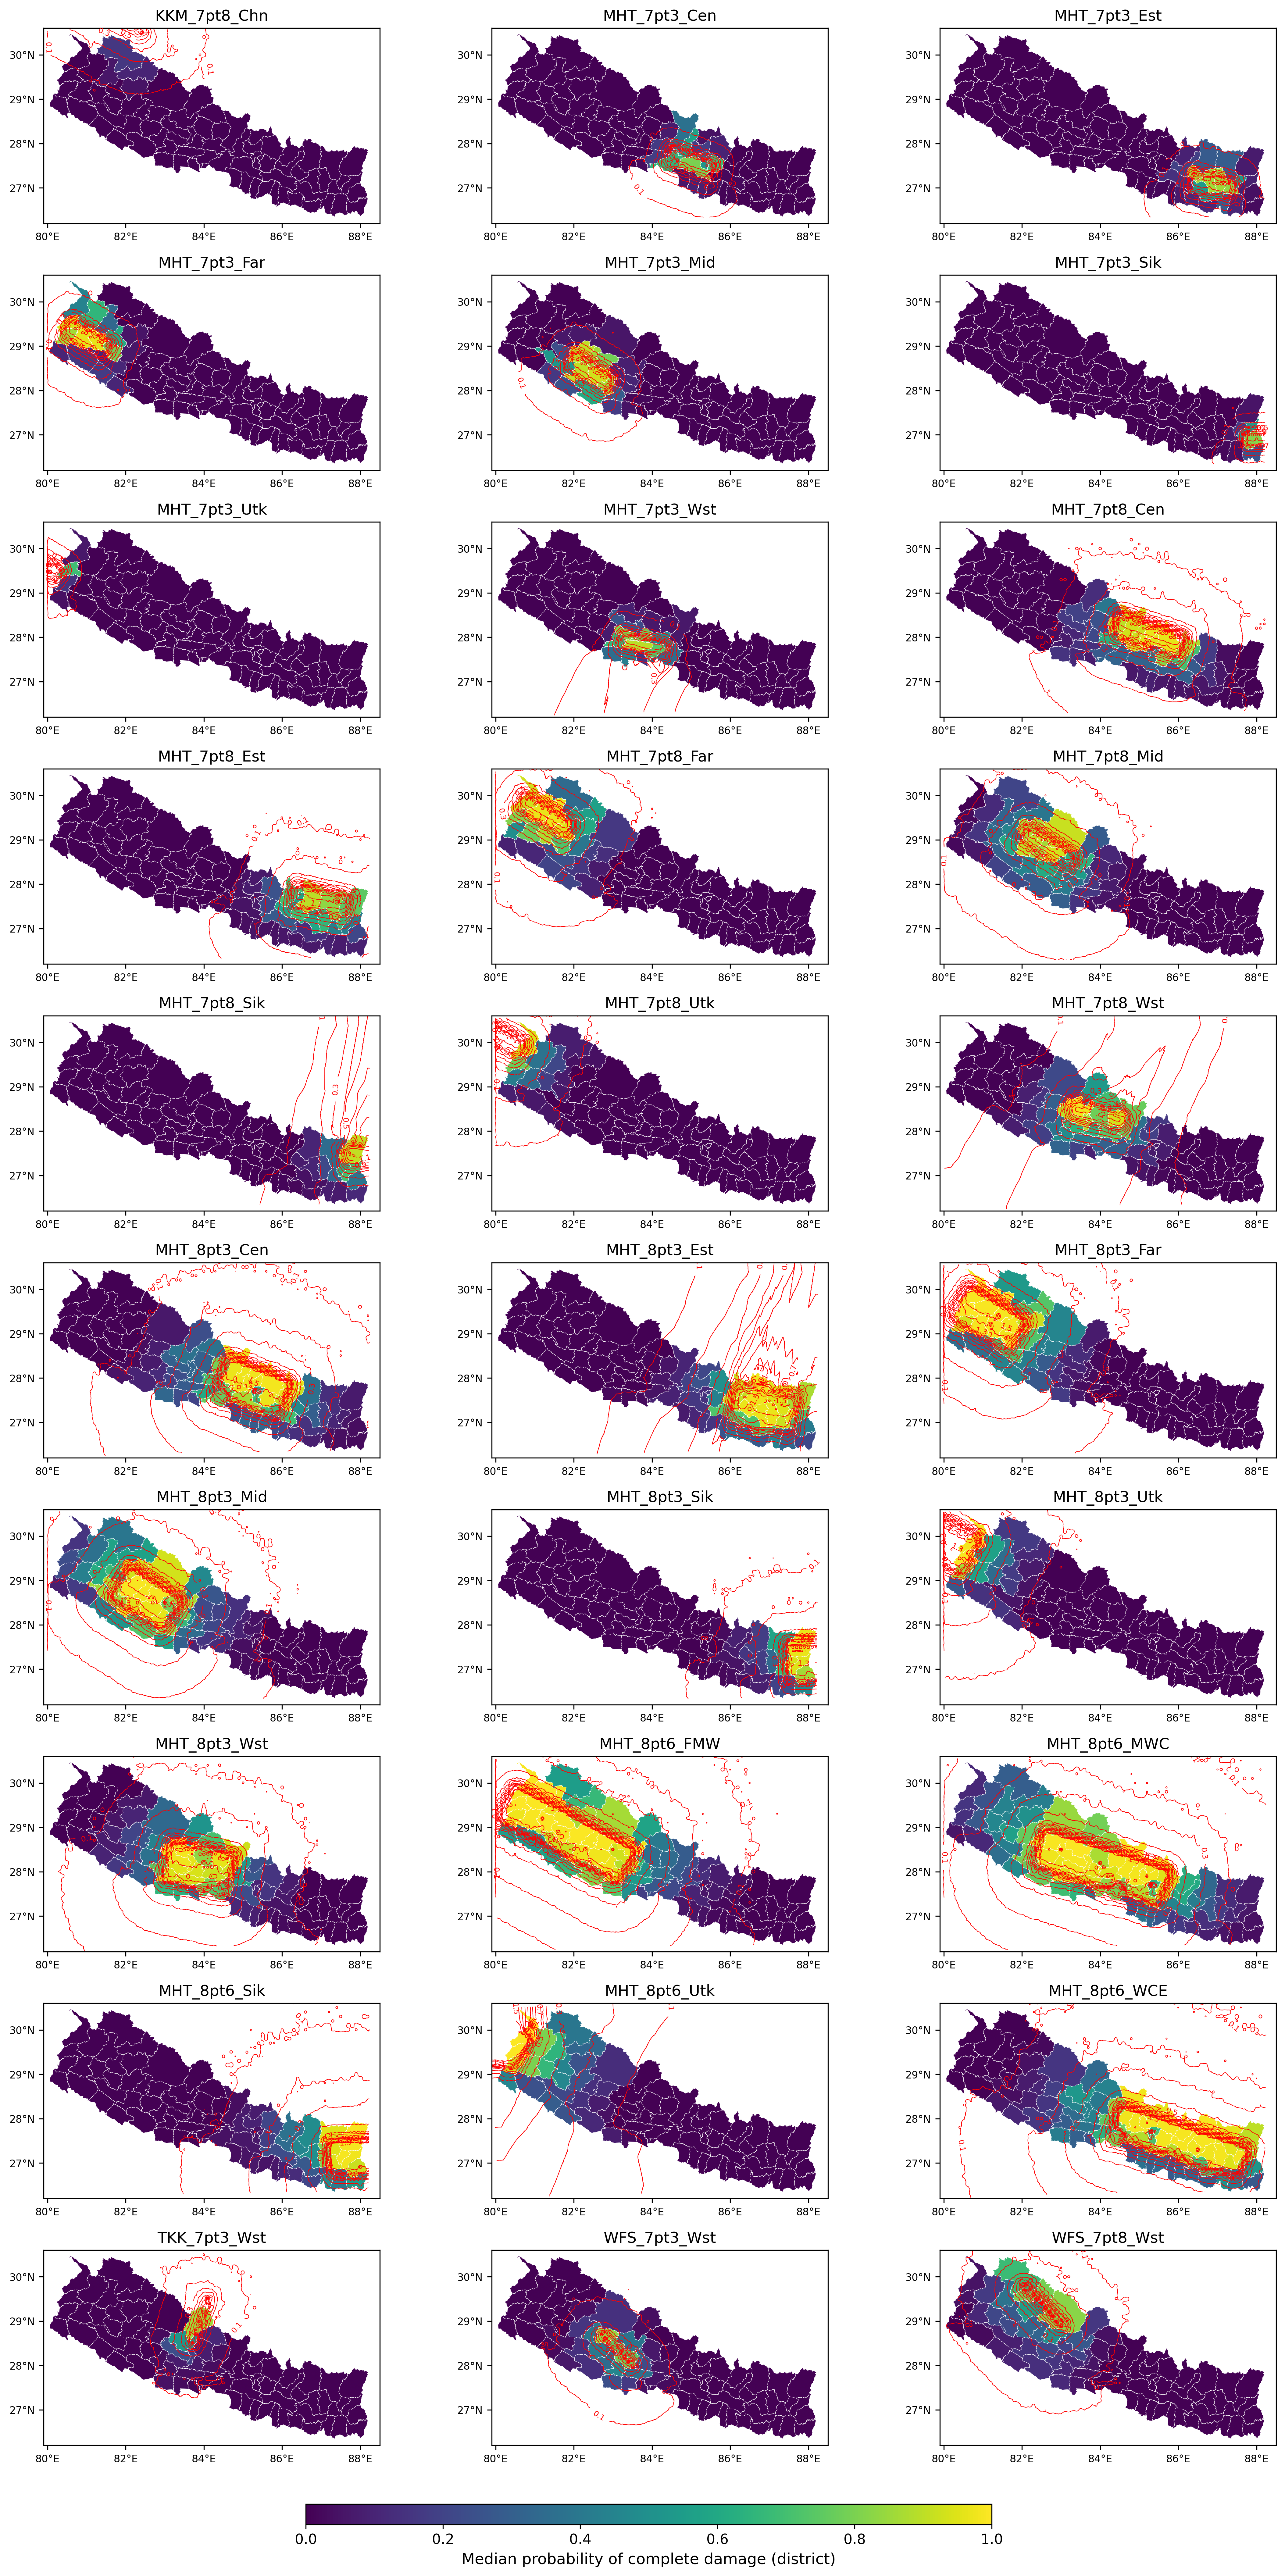
\includegraphics[width=\textwidth,height=0.82\textheight,keepaspectratio]{figures/figS3.png}
\caption{Maps of the median probability of complete damage in each district for each of the 30 scenario earthquakes in the ensemble. The probability of complete damage is modelled for each $90 \times 90$~m grid cell of the METEOR exposure dataset using the middle-case fragility functions (Fig.~\ref{fig:S1}), and the median of these cell values is shown for each district \citep{Dunant2025}. Red contours show peak ground acceleration (PGA, in g).}
\label{fig:S3}
\end{figure}

\begin{figure}[p]
\centering
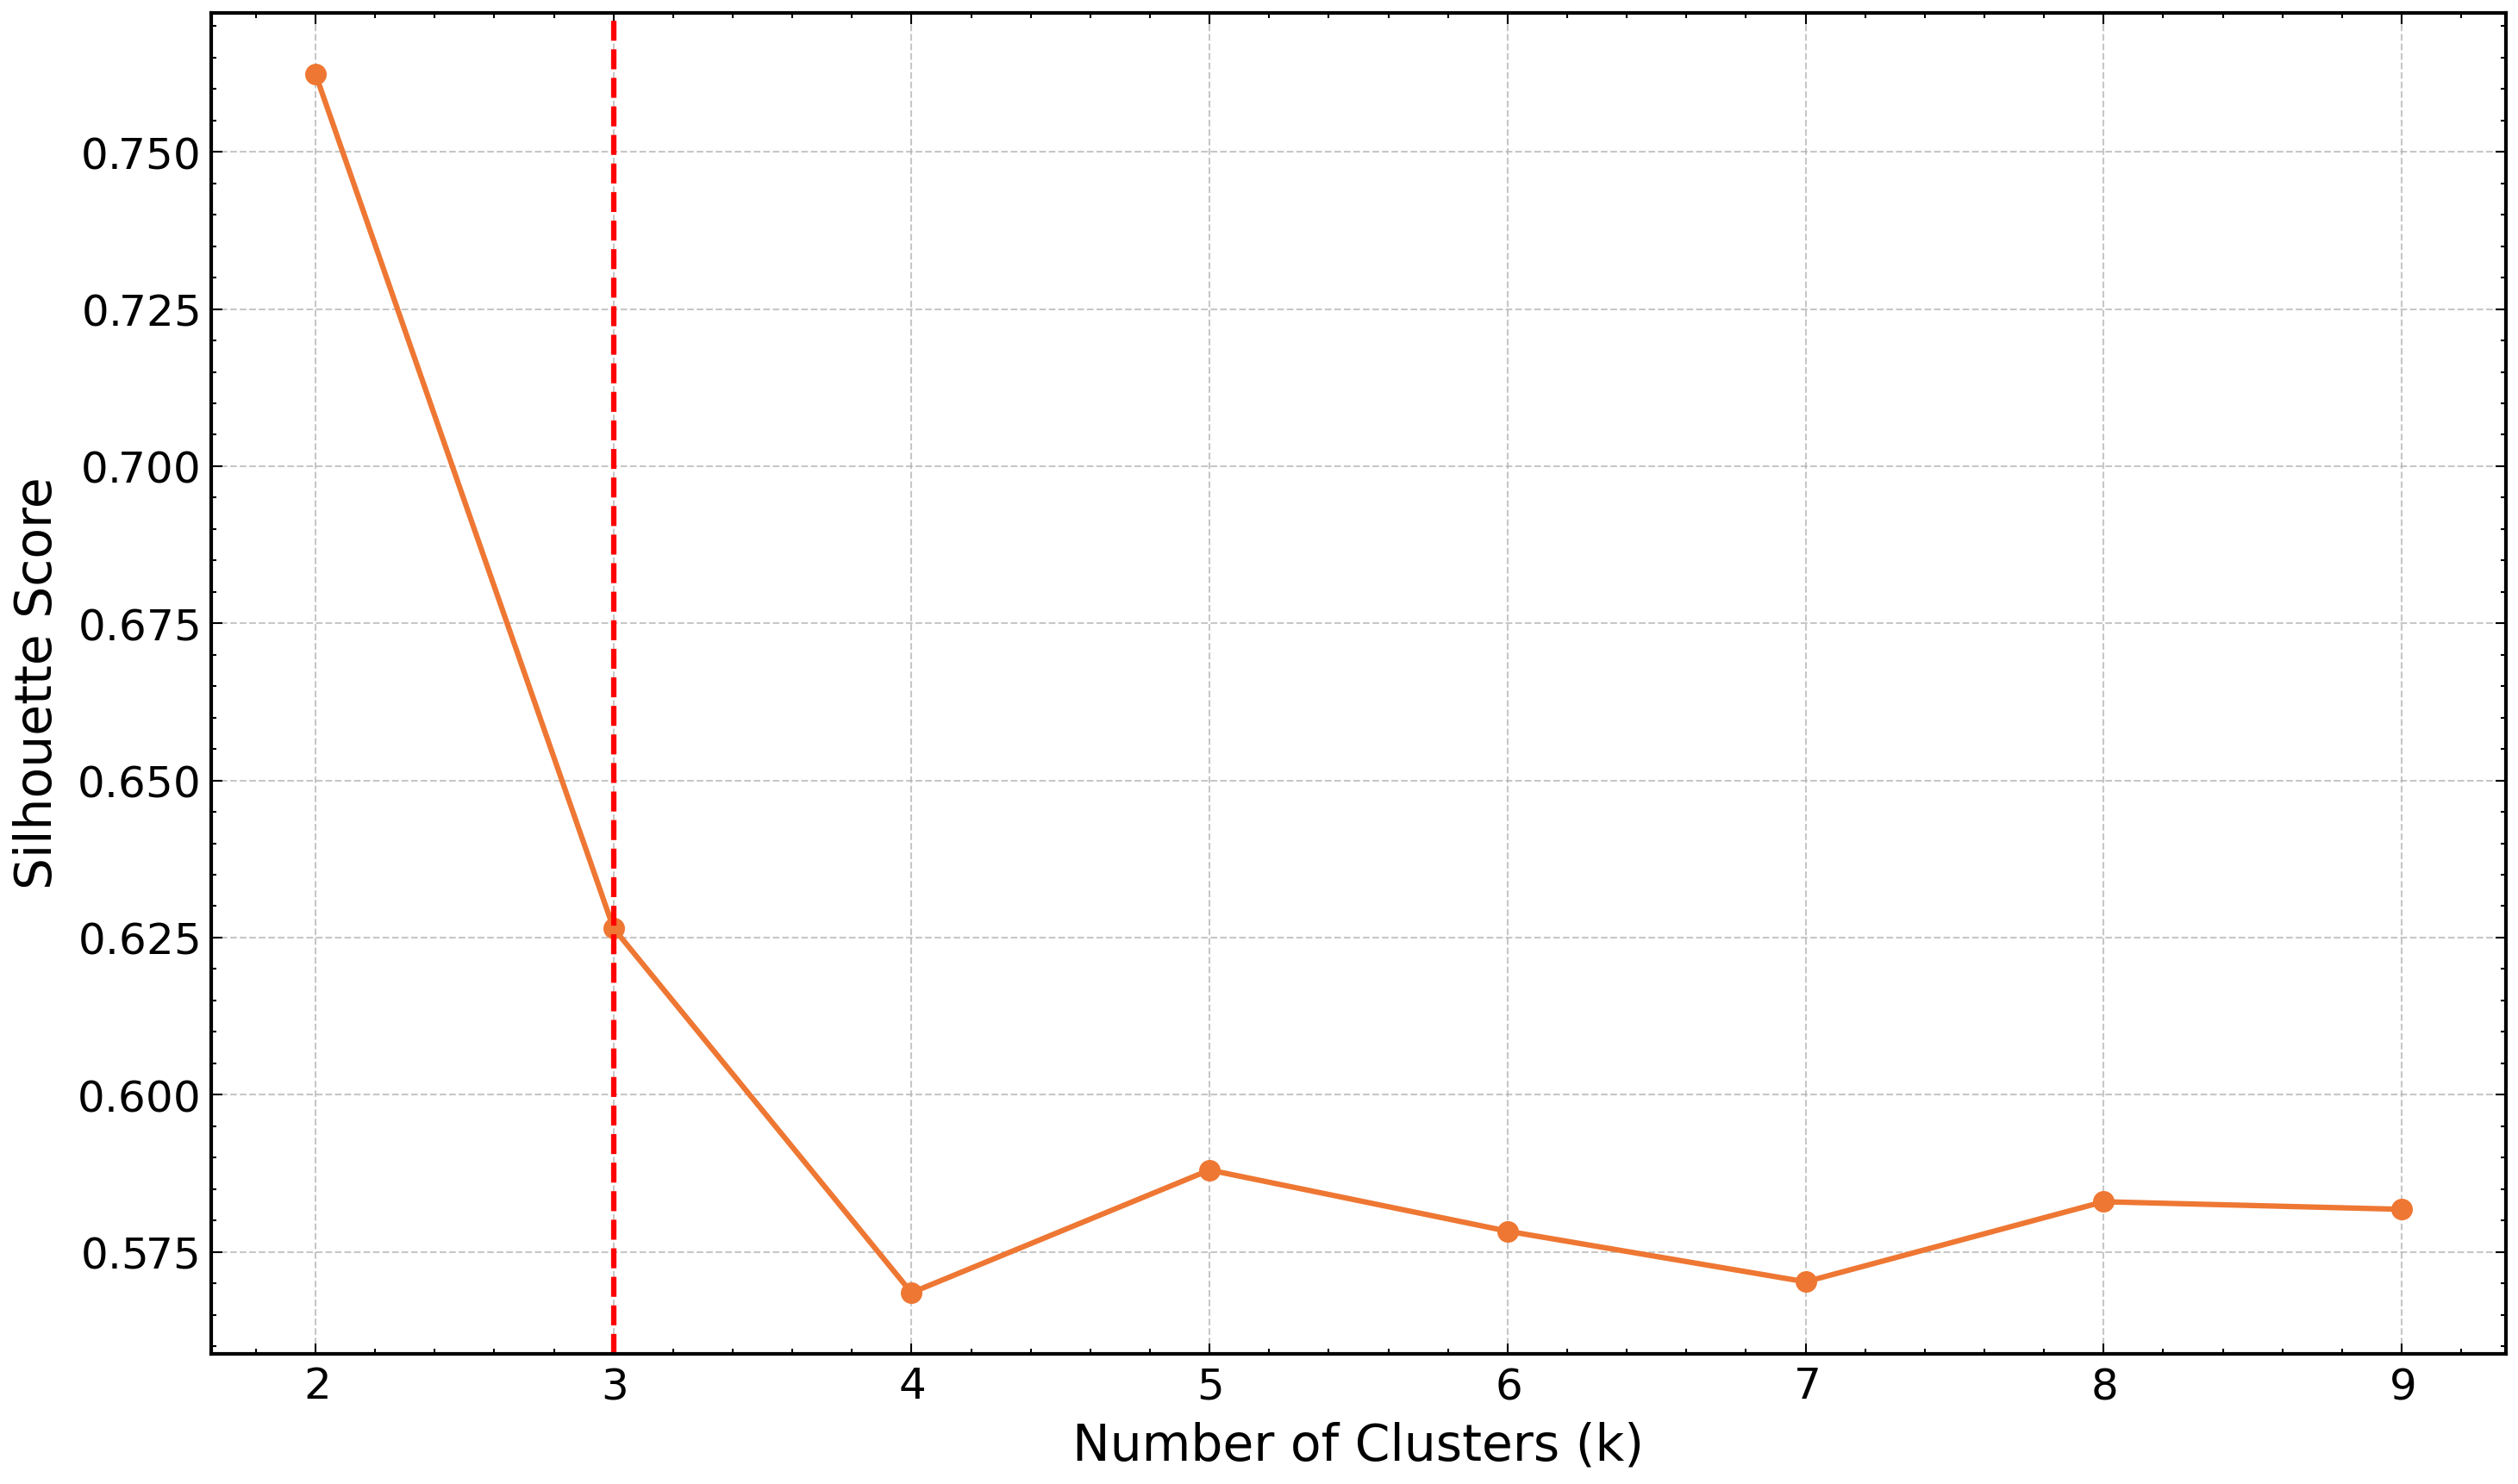
\includegraphics[width=\textwidth]{figures/figS4.png}
\caption{Silhouette scores for K-means clustering of the district remoteness index (access to district headquarters, dry season) with $k = 2$--9 clusters. The dashed line marks the three clusters retained for interpretability.}
\label{fig:S4}
\end{figure}

\begin{figure}[p]
\centering
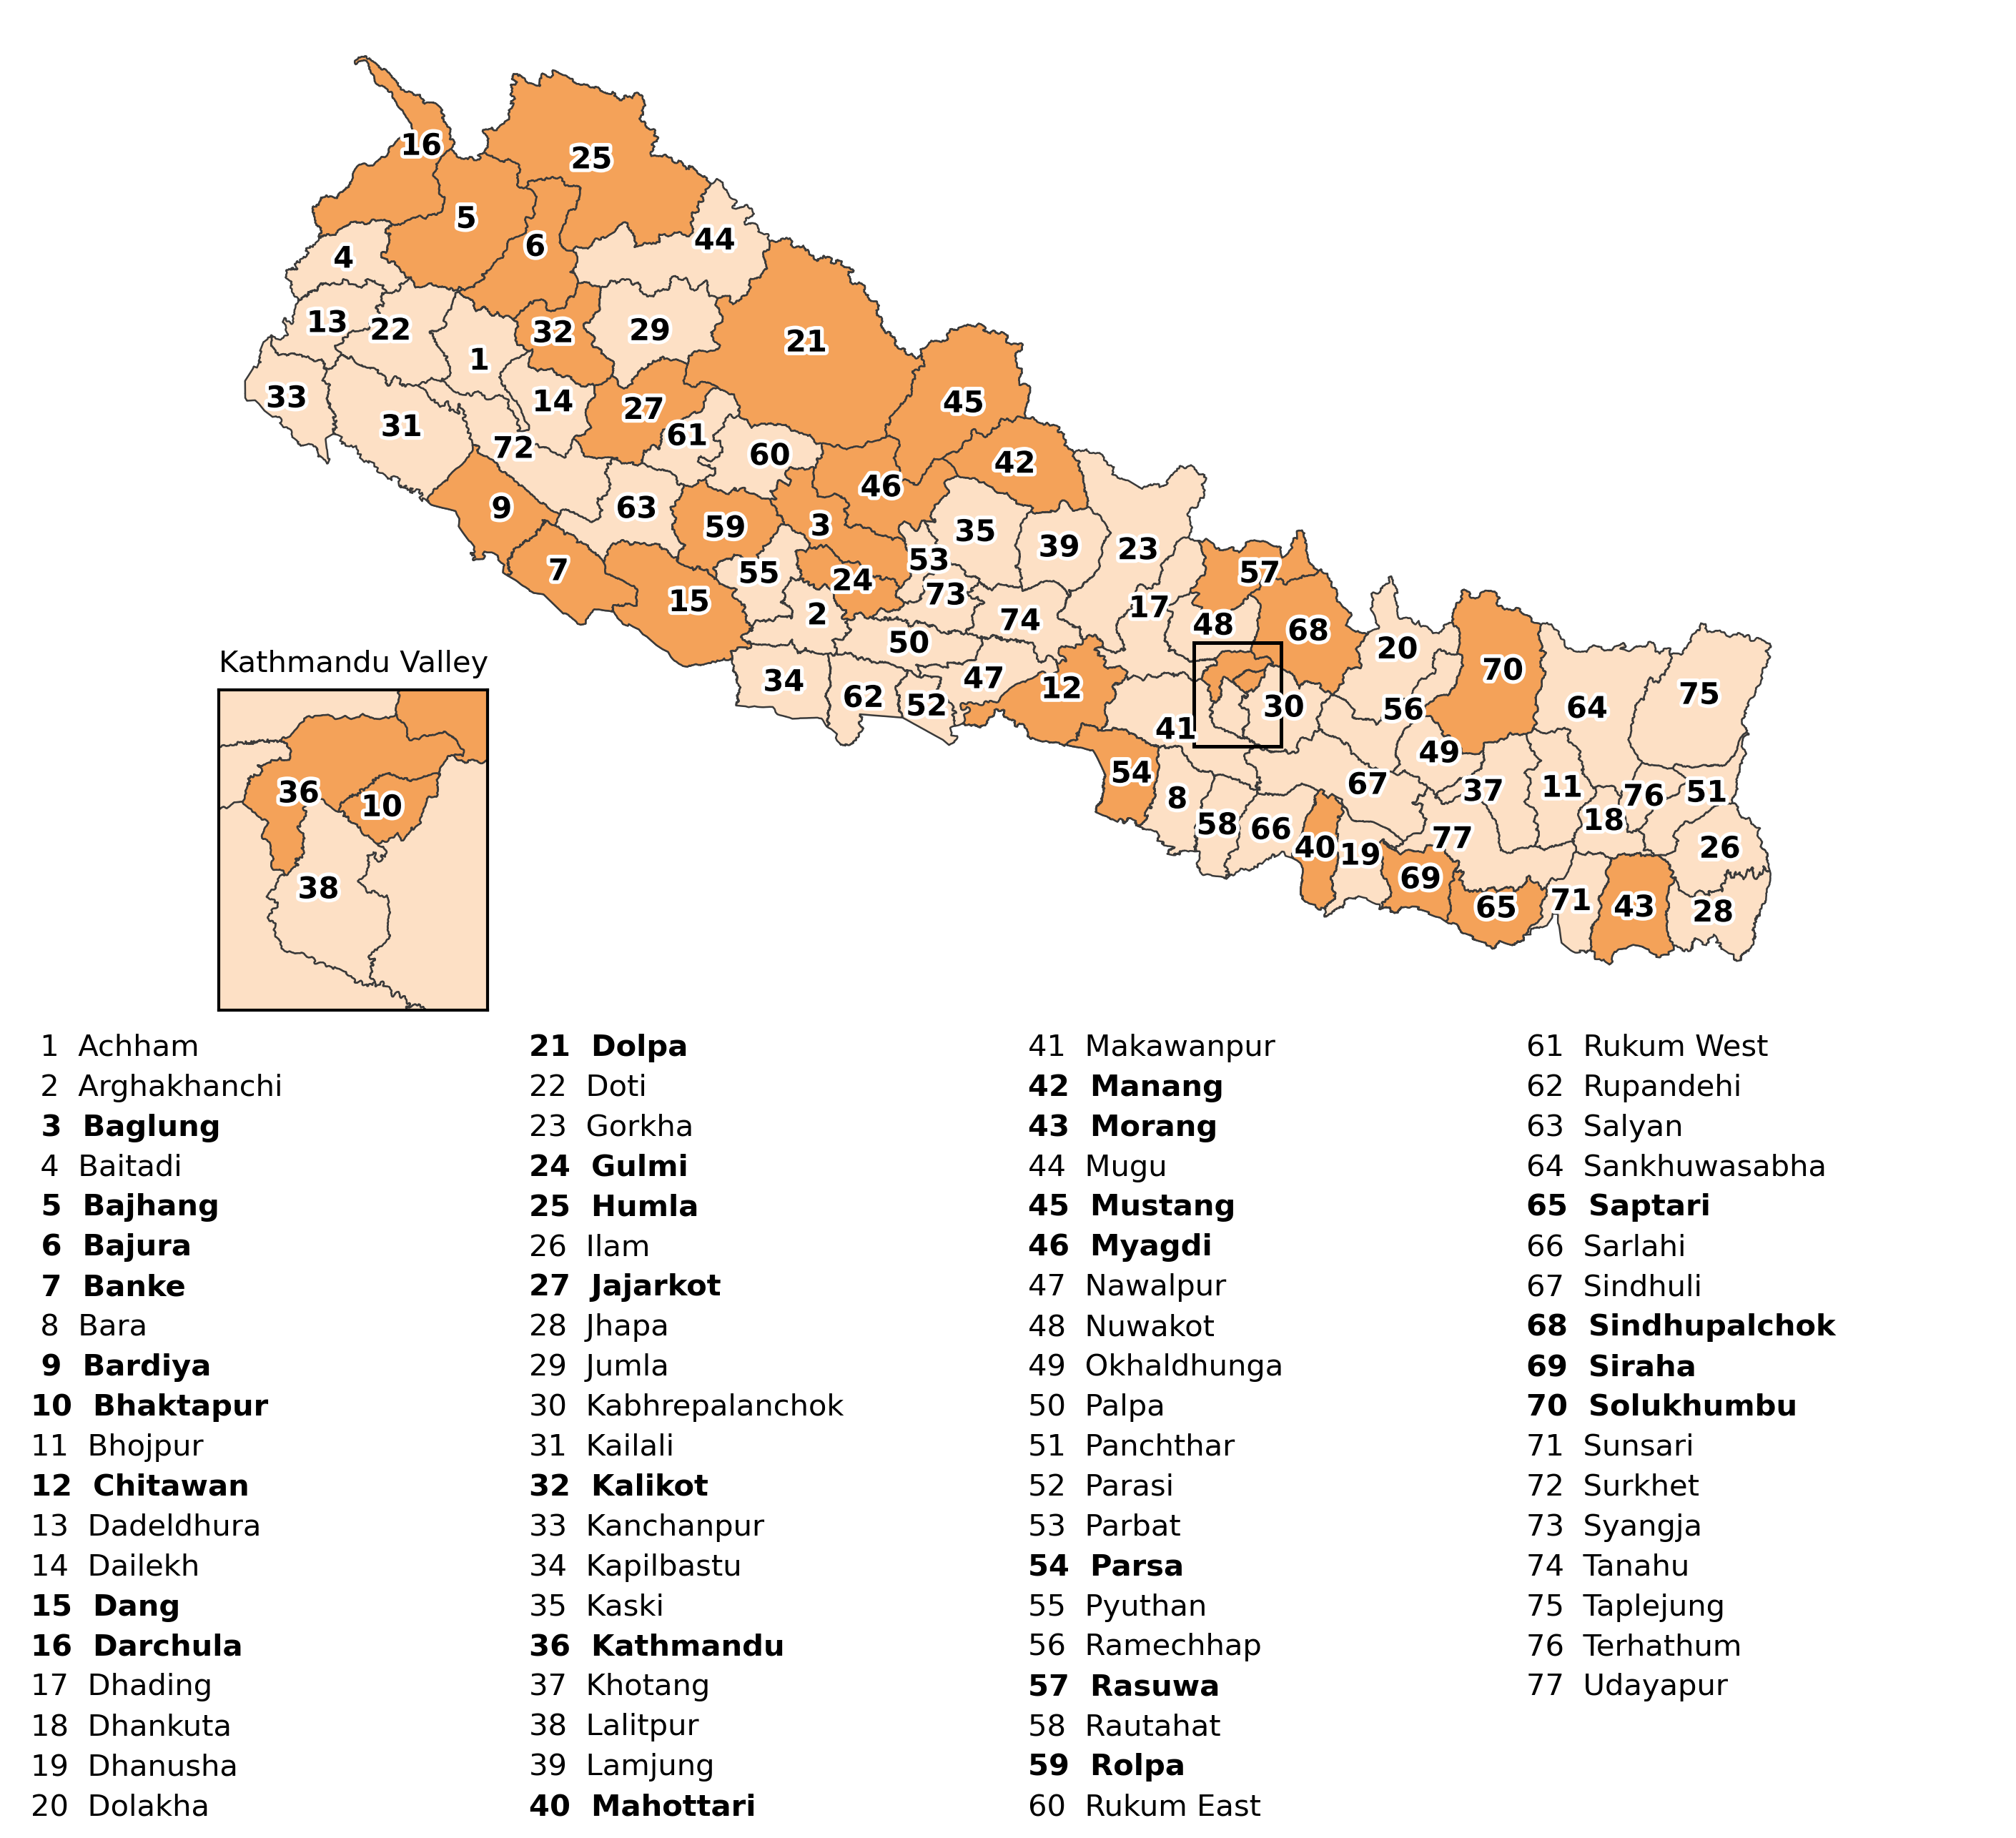
\includegraphics[width=\textwidth,height=0.82\textheight,keepaspectratio]{figures/figS5.png}
\caption{Names and outlines of the 77 districts of Nepal used in this study.}
\label{fig:S5}
\end{figure}

\clearpage

\begin{table}[t]
\centering
\caption{Sensitivity of the district rankings to the weights in the risk scores. Each alternative is compared with the score used in the main text (Eqs.~2 and 3 of the main text): Spearman rank correlation across the 77 districts, largest change in the rank of any district, and number of districts shared by the two lists of the ten highest-ranked districts. For the absolute score, the road-segment weight sets how many buildings one damaged 100~m road segment counts as (1 in the main text); R/S/L are the weights of remoteness, shaking and landslides in the normalised score (0.50/0.25/0.25 in the main text).}
\label{tab:S1}
\begin{tabular}{lccc}
\toprule
            & Spearman & Max.\ rank & Top-10  \\
Alternative & $\rho$   & shift      & overlap \\
\midrule
\multicolumn{4}{l}{\textit{Absolute score}} \\
\quad Buildings only (no roads) & 0.998 & 5  & 9  \\
\quad Road segment = 0.5 bldg.  & 0.999 & 3  & 9  \\
\quad Road segment = 2 bldgs.   & 0.997 & 5  & 10 \\
\quad Remoteness weight 0.4     & 0.969 & 15 & 8  \\
\quad Remoteness weight 0.6     & 0.966 & 16 & 6  \\
\addlinespace
\multicolumn{4}{l}{\textit{Normalised score (R/S/L)}} \\
\quad 0.33/0.33/0.33 & 0.993 & 9 & 8  \\
\quad 0.40/0.30/0.30 & 0.997 & 6 & 9  \\
\quad 0.60/0.20/0.20 & 0.998 & 5 & 9  \\
\quad 0.50/0.35/0.15 & 0.997 & 6 & 10 \\
\quad 0.50/0.15/0.35 & 0.998 & 4 & 10 \\
\bottomrule
\end{tabular}
\end{table}

\begin{table}[t]
\centering
\caption{Districts whose rank in the normalised risk score changes by at least eight places when the landslide term is added to a shaking-only version of the score (rank 1 = highest risk among 77 districts). Positive changes indicate a higher ranking once landslides are included.}
\label{tab:S2}
\begin{tabular}{lccc}
\toprule
District & Rank, shaking only & Rank, shaking + landslides & Change \\
\midrule
Rasuwa & 36 & 14 & +22 \\
Baglung & 33 & 21 & +12 \\
Myagdi & 31 & 19 & +12 \\
Gulmi & 41 & 33 & +8 \\
Jumla & 10 & 18 & $-8$ \\
Salyan & 20 & 29 & $-9$ \\
Dhading & 24 & 34 & $-10$ \\
Bhojpur & 26 & 36 & $-10$ \\
Dadeldhura & 22 & 35 & $-13$ \\
\bottomrule
\end{tabular}
\end{table}

\clearpage

\bibliographystyle{copernicus}
\bibliography{references}

\end{document}
